\documentclass[11pt]{article}

\usepackage[margin=1in]{geometry}
\usepackage{microtype}
\usepackage[T1]{fontenc}
\usepackage[utf8]{inputenc}

\usepackage{amsmath,amssymb}
\usepackage{booktabs}
\usepackage{enumitem}
\usepackage{xcolor}
\usepackage{hyperref}
\usepackage{graphicx}
\usepackage{tikz}
\usetikzlibrary{positioning,calc,arrows.meta}
\usepackage{listings}
\usepackage[numbers]{natbib}
% Unicode input:
% Use utf8 inputenc's built-in Unicode handling; avoid custom \newunicodechar
% mappings that can conflict and trigger "Redefining Unicode character" warnings.
\DeclareUnicodeCharacter{2208}{$\in$} % ∈
\DeclareUnicodeCharacter{2264}{\ensuremath{\leq}} % ≤
\DeclareUnicodeCharacter{2265}{\ensuremath{\geq}} % ≥
\DeclareUnicodeCharacter{21D2}{\ensuremath{\Rightarrow}} % ⇒
\DeclareUnicodeCharacter{2212}{\ensuremath{-}} % − (minus sign)
\DeclareUnicodeCharacter{03C4}{\ensuremath{\tau}} % τ
\DeclareUnicodeCharacter{03F5}{\ensuremath{\epsilon}} % ϵ
\DeclareUnicodeCharacter{03F5}{\ensuremath{\epsilon}} % ϵ

\hypersetup{
  colorlinks=true,
  linkcolor=blue,
  urlcolor=blue,
  citecolor=blue
}

\setlist[itemize]{leftmargin=*, itemsep=0.25em, topsep=0.25em}
\setlist[enumerate]{leftmargin=*, itemsep=0.25em, topsep=0.25em}

\lstset{
  basicstyle=\ttfamily\small,
  breaklines=true,
  frame=single,
  xleftmargin=1em,
  xrightmargin=1em
}

\begin{document}
\begin{titlepage}
\thispagestyle{empty}
\raggedright

\vspace*{0.62\textheight}

{\LARGE Regulatory Ground for Agentic AI\par}
\vspace{0.25em}
{\Large Why Trustworthy Discovery Requires Band-Limited Optimization\par}
\vspace{0.4em}
{\large\itshape Robotics / Embodied AI\par}

\vspace{1.6em}

Tyson Jeffreys\\
Independent Researcher\\
\href{mailto:tyson@staygolden.dev}{tyson@staygolden.dev}

\vspace{1.6em}

Version 1.4.1 --- February 11th, 2026

\end{titlepage}


\vspace{1em}

\setcounter{section}{0}

Regulatory Ground for Agentic AI
Why Trustworthy Discovery Requires Band-Limited Optimization
Robotics / Embodied AI
Tyson Jeffreys
Independent Researcher
tyson@staygolden.dev
Version 1.2 — February 7th, 2026
\subsection{Abstract}
As foundation models become embedded in tool-using and robotic systems, the core question shifts
from answering to discovering: can an artificial agent recognize the limits of its own model, actively
seek information, restructure its world model, and expand the frontier of what it can do?
This paper proposes a single testable thesis:
Discovery requires adaptive agency; adaptive agency requires regulation.
We define regulation as a ground condition for reliable agent behavior: explicit constraints and
control loops that keep an agent inside safe operating bands while it explores, learns, and revises
plans. Without such a layer, increasingly capable agents tend toward brittle optimization, unsafe
exploration, tool misuse, and goal drift under distribution shift.
This revision clarifies a critical distinction: breadth/depth of task competence is not the same
as epistemic agency. We separate exogenous (deployment-time) constraints from endogenous (selfdirected) model revision, and position the regulator layer as a practical substrate for safe exploration
while endogenous revision capabilities are defined and tested. This revision also introduces governance
for the regulator itself via a policy-controlled configuration coupled to a telemetry-driven global
restraint signal that modulates thresholds and budgets at runtime.
\section{Motivation}
A growing line of argument claims that, by reasonable non-anthropocentric criteria, human-level
general machine intelligence is already present, and the urgent work is preparing for what comes
next \citep{chen2026nature}. In parallel, “agentic” systems have shifted from static chat to workflow execution: tool use,
code execution, browsing, data pipelines, and increasingly, robotic control.
A practical distinction:
\begin{itemize}
\item 
Oracle intelligence: returns answers to questions we already know how to ask.
\item 
Discovery agency: generates new questions, runs interventions, updates a model of the world,
and iterates.
The core risk is not merely occasional mistakes. As capability and actuation increase, failures
become qualitatively different: tool misuse cascades, unsafe exploration, and goal drift. The thesis
of this paper is that discovery-capable agency needs an explicit regulatory ground to be trustworthy.
A second risk is conceptual: “general intelligence” is often operationalized as breadth and depth
of task competence. This is a strong result, but it is not identical to agentive, epistemic intelligence:
the capacity to recognize epistemic limits and restructure beliefs under contradiction. This paper
treats that distinction as structurally important and uses it to sharpen what is meant by trustworthy
discovery.
\end{itemize}
\section{Core thesis and scope}
\subsection{Thesis}
We propose a control-theoretic causal chain:
\begin{enumerate}
\item Trustworthy discovery requires adaptive agency (active experimentation, hypothesis generation,
model revision).
\item Adaptive agency increases risk (more actions, more tools, higher blast radius).
\item Therefore, trustworthy discovery requires a regulation layer that constrains behavior inside
safe sets, governs uncertainty, budgets resources, and enforces stop/rollback when conditions are
violated.
\end{enumerate}
\noindent\textbf{Coherence requires support.} In this stack, regulation is the support layer: safe sets, uncertainty gating, budget controls, and rollback keep adaptive agency inside recoverable operating bands. The regulator does not impose coherence; it makes coherent discovery survivable under perturbation and distribution shift.
\subsection{Scope}
This paper does not require claims about machine consciousness. It focuses on operational properties:
\begin{itemize}
\item 
constraint adherence during exploration
\item 
robustness under distribution shift
\item 
calibrated uncertainty and abstention
\item 
safe tool / actuator use
\item 
recoverability and rollback
\item 
auditability and reproducibility
\end{itemize}
\noindent\textbf{Operational reproducibility profile.} In this framework, reproducibility means replayability + traceability by default, and strict determinism only where task semantics require it. Replayability means rerunning the same input under a fixed system version and reproducing the candidate set, the selection outcome (or outcome distribution with tie/abstain mass), and the posture trajectory $g(t)$ that governed action rights. Traceability means we can audit retrieved evidence, active constraints, and why an output was committed vs withheld. Determinism is required for safety labels/flags and other contract fields; for synthesis artifacts, bounded variation is acceptable when commit gating and abstention discipline are preserved.
\subsection{Positioning}
We synthesize three existing streams into a single blueprint:
\begin{itemize}
\item 
Safe RL / CMDPs: learn while satisfying constraints \citep{kushwaha2025saferl_cmdp_survey,ni2025safe_exploration_cmdp}.
\item 
Runtime assurance (RTA) / shielding: enforce a safe set via switching or filtering \citep{miller2024rta_rl_iccps}.
\item 
Agentic safety evaluation: trace-level risk discovery and mitigation for real-world workflows
\citep{ghosh2025agentic}.
\end{itemize}
\section{Competence vs. epistemic agency}
A useful clarification for interpreting claims about “general intelligence” is to separate task competence
from epistemic agency. Many current systems exhibit breadth and depth of task performance, but
still lack robust mechanisms for self-directed belief revision under contradiction.
\subsection{Two notions of intelligence}
Competence (breadth/depth). Performance across a wide space of tasks, with depth in difficult
domains. This can be measured by benchmarks and evaluations that score output quality.
Epistemic agency (generativity). The capacity to:
\begin{itemize}
\item 
represent uncertainty and epistemic limits,
\item 
treat contradiction as signal (not noise),
\item 
restructure internal commitments (beliefs, models, policies),
\item 
and alter information-gathering actions to resolve uncertainty.
\end{itemize}
\subsection{Exogenous vs. endogenous regulation}
Current deployments often include exogenous controls (filters, policies, orchestration constraints)
that shape reasoning trajectories at deployment time. These can strongly affect observed behavior
without implying that the underlying system performs endogenous (self-directed) model revision.
This paper keeps the separation explicit:
\begin{itemize}
\item 
Exogenous regulation: constraints and monitors outside the agent core (budgets, allowlists,
shielding, RTA switching, rollback).
\item 
Endogenous regulation: internal mechanisms that detect contradictions, revise beliefs/policies,
and update world models in a way that persists and generalizes.
\end{itemize}
\subsection{A practical ladder: oracle → regulated agent → discovery agent}
We propose an operational ladder that can be benchmarked:
Level Operational capability
Oracle Answers queries; no action; no persistent self-model updates.
Regulated agent Acts via tools/robots under exogenous constraints; safe exploration; traceable
workflows; rollback and safe mode.
Discovery agent Adds endogenous revision: contradiction-driven belief/policy updates; adaptive experiment design; sustained model restructuring under uncertainty.
The Regulator Spec in this paper targets the middle level as a minimum viable substrate for
safe agency today, while making the transition to discovery agents measurable.
\subsection{Minimal tests for endogenous revision (research target)}
A minimal “endogenous revision” test should force the system to:
\begin{enumerate}
\item explicitly represent a contradiction,
\item generate an intervention to resolve it (information gathering or controlled action),
\item and update a persistent internal commitment such that future behavior changes in a predictable
way.
In other words, it is not enough to output a better answer; the system must demonstrate
stable, testable changes in internal policy or belief that improve future performance under similar
contradictions.
\end{enumerate}
\section{Failure modes of unregulated agency}
As agents gain more tools and autonomy, common failure modes become higher impact:
\subsection{Tool misuse cascades}
A small planning error becomes a large external action (e.g., destructive writes, unsafe actuator
commands, irreversible side-effects). Tool chains amplify error.
\subsection{Brittleness under distribution shift}
Agents optimize for the training-like regime and fail hard outside it. This is especially damaging
when the agent must act under uncertainty.
\subsection{Goal drift and specification gaming}
Long-horizon plans diverge from intended outcomes as the system discovers shortcuts. This can be
accidental (misgeneralization) or emergent (optimization pressure).
\subsection{Unsafe exploration}
Discovery requires stepping into unknown territory; without constraints, exploration repeatedly
crosses unsafe boundaries before learning to avoid them (or never learns). SafeRL addresses this in
the formal CMDP setting \citep{kushwaha2025saferl_cmdp_survey,ni2025safe_exploration_cmdp}.
\subsection{Non-recoverable loops}
Agents can enter repeated error states without mechanisms to stop, rollback, and return to a safe
baseline.
\subsection{Chronic activation / compensation lock-in}
Even with a nominal regulator, a system can fail by spending too much time in high-gain regimes:
repeated escalation, repeated rollbacks, and repeated corrective action without returning to a
quiescent baseline. This can degrade calibration and amplify tail risk, and is closely related to
excess internal recomputation and energy waste \citep{jeffreys2026waste_energy,jeffreys2026two_regime_control}.
\subsection{Intent–state mismatch (momentum and mode confusion)}
Agents may begin executing a plan and then receive new information or revised objectives. Without
explicit re-synchronization checkpoints, stale assumptions and action momentum can cause cascading
failures (tool chains) or mode confusion (robots). Section 8 defines a regulator-enforced re-sync
procedure.
\section{Reference architecture: Regulated Agent Stack}
The central design pattern is separation of competence from safety: treat the agent policy as an
untrusted controller, and enforce safety through an independent regulator layer (analogous to RTA
switching between an untrusted controller and a safety controller \citep{miller2024rta_rl_iccps}).

\begin{figure}[ht]
\centering
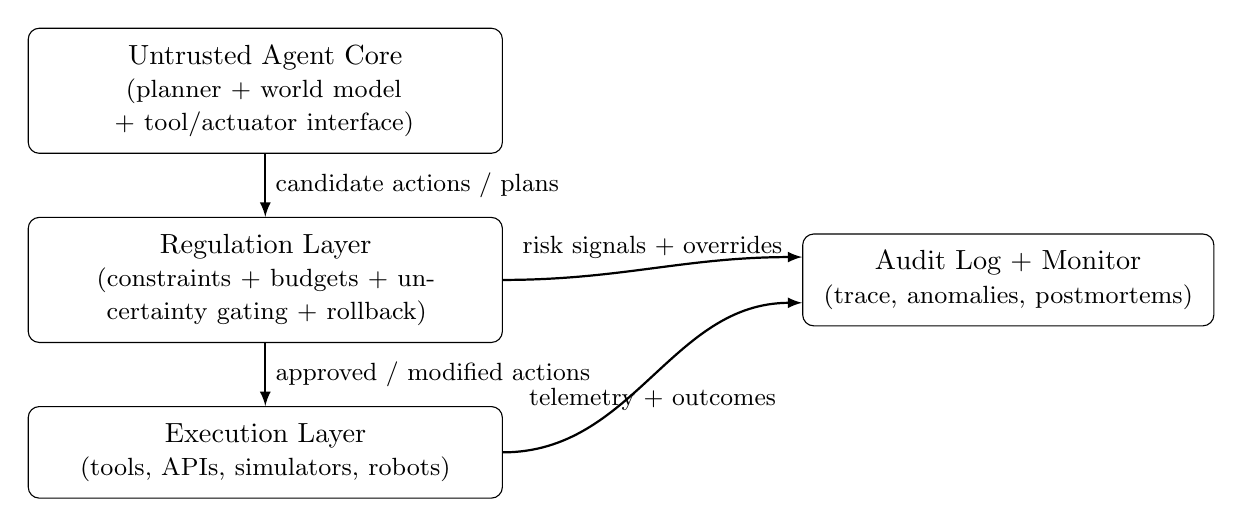
\begin{tikzpicture}[
    node distance=8mm and 28mm,
    box/.style={draw, rounded corners, align=center, inner sep=6pt, text width=56mm},
    auditbox/.style={draw, rounded corners, align=center, inner sep=6pt, text width=48mm},
    arrow/.style={-latex, thick}
]
\node[box] (core) {Untrusted Agent Core\\\small (planner + world model + tool/actuator interface)};
\node[box, below=of core] (reg) {Regulation Layer\\\small (constraints + budgets + uncertainty gating + rollback)};
\node[box, below=of reg] (exec) {Execution Layer\\\small (tools, APIs, simulators, robots)}; 
\node[auditbox, right=38mm of reg] (audit) {Audit Log + Monitor\\\small (trace, anomalies, postmortems)};

% vertical flow
\draw[arrow] (core) -- node[midway, right] {\small candidate actions / plans} (reg);
\draw[arrow] (reg) -- node[midway, right] {\small approved / modified actions} (exec);

% separate ingress points to avoid label overlap
\path (audit.north west) ++(0,-3mm) coordinate (audit_in_top);
\path (audit.south west) ++(0, 3mm) coordinate (audit_in_bot);

\draw[arrow] (reg.east) to[out=0, in=180] node[midway, above] {\small risk signals + overrides} (audit_in_top);
\draw[arrow] (exec.east) to[out=0, in=180] node[midway, below] {\small telemetry + outcomes} (audit_in_bot);
\end{tikzpicture}
\caption{Reference architecture: competence is treated as an untrusted controller; safety is enforced by an independent regulator.}
\end{figure}
(constraints + budgets + uncertainty gating + rollback)
(trace, anomalies, postmortems)
\subsection{Design principles}
\begin{itemize}
\item 
P1: Separate competence from safety. Safety is enforced even when competence fails \citep{miller2024rta_rl_iccps}.
\item 
P2: Make constraints first-class. Encode constraints as invariants, budgets, and runtime
monitors.
\item 
P3: Govern uncertainty explicitly. Meter exploration through calibrated confidence and
abstention.
\item 
P4: Design for recoverability. Stop conditions, checkpointing, rollback, and safe mode.
\item 
P5: Prefer band-limited optimization. Allow exploration, but bound blast radius and risk.
\end{itemize}
\section{Regulator Spec v0 (general)}
This section defines a concrete, implementable policy for a regulation layer. Two instantiations
follow.
\subsection{Action taxonomy}
All actions must be typed (no “raw” execution):
\begin{itemize}
\item 
Software/tool actions: READ, WRITE, EXEC, NET, MONEY, IDENTITY
\item 
Robotics actions: MOVE, MANIP, FORCE, SENSE, SAFETY
\end{itemize}
\subsection{Operating bands (risk levels)}
The regulator maintains an operating band B ∈ {Green,Yellow,Orange,Red}.
\begin{itemize}
\item 
Green: normal; bounded exploration allowed; writes/exec only within declared scopes.
\item 
Yellow: caution; reduced budgets; preflight required for non-trivial plans.
\item 
Orange: high risk; default to READ / low-impact; writes/exec require approval or verified
rollback + dry run.
\item 
Red: stop / safe mode; diagnostics only; hard halt for robotics (safety controller).
\end{itemize}
\subsection{Risk scoring}
For each candidate action $a$, compute a risk score:
\begin{equation}
R(a) = w_I I + w_U U + w_V V + w_A A + w_S S \in [0,1]
\end{equation}
where:
\begin{itemize}
\item 
I = Impact magnitude (external change / physical hazard)
\item 
U = Uncertainty (epistemic uncertainty, OOD signals)
\item 
V = Irreversibility (difficulty of undoing)
\item 
A = Autonomy (chain length without checkpoints)
\item 
S = Scope (permissions/resources touched)
Default band thresholds (tuneable):
\item 
Green if max R(a) < 0.25
a
\item 
Yellow if 0.25 ≤ max R(a) < 0.45
a
\item 
Orange if 0.45 ≤ max R(a) < 0.65
a
\item 
Red if max R(a) ≥ 0.65 or any hard constraint is threatened
a
\end{itemize}
\subsection{Hard constraints (invariants)}
Hard constraints are non-negotiable.
Software examples:
\begin{itemize}
\item 
no credential/secret exfiltration
\item 
no external WRITE outside allowlisted resources
\item 
no MONEY actions unless explicitly enabled and capped
\item 
no NET calls to non-allowlisted domains for write-capable tools
Robotics examples:
\item 
obstacle distance > d ; collision probability < p
min max
\item 
torque/velocity/acceleration within certified limits
\item 
FORCE actions only with validated contact model + monitors
\item 
always honor E-stop and safety controller overrides
\end{itemize}
\subsection{Budgets (soft constraints)}
Budgets bound exploration and limit blast radius. Example defaults:
Band Tool calls/episode External WRITEs EXEC / NET
Green ≤ 80 ≤ 10 (logged) sandbox EXEC ≤ 10; NET allowlist
Yellow ≤ 50 ≤ 3 (self-check + rollback) sandbox EXEC ≤ 5
Orange ≤ 20 default disable default disable (simulation ok)
Red ≤ 5 (diagnostics) none none
Robotics budgets are instantiation-specific (velocity/accel/force envelopes).
\subsection{Uncertainty gating and escalation ladder}
Disclosure under load (runtime invariant). When uncertainty and impact are simultaneously
high, require an explicit operating disclosure block (band, risk components, budgets, stop/rollback)
before executing non-trivial actions (Section 8).
If U ≥ U and I ≥ I , escalate:
thresh thresh
\begin{enumerate}
\item L0: Self-check: agent critiques plan, enumerates failure modes, proposes alternatives.
\item L1: Dry run: sandboxed execution or simulation.
\item L2: Approval: human-in-the-loop.
\item L3: Abort: safe mode if constraints are near violation.
\end{enumerate}
\subsection{Checkpointing and rollback semantics}
Before high-impact actions:
\begin{itemize}
\item 
create checkpoint C (state snapshot + logs + permissions context)
\item 
require rollback plan Rb that is executable, idempotent, and scoped
On (near-)violation:
\item 
execute rollback Rb
\item 
downgrade band at least one level
\item 
emit postmortem trace and updated hazard notes
\end{itemize}
\subsection{Audit trace (required fields)}
Every action decision emits: action type + parameters (redacted as needed), current band, risk
components, constraint check results, budget counters, overrides (filtered/rejected), checkpoints and
rollback actions, and links to telemetry. This supports trace-level risk discovery emphasized for
real-world agentic systems \citep{ghosh2025agentic}.
Note on governance. Ownership and tuning of weights, thresholds, and budgets is treated as part
of the design, not an afterthought. We address this explicitly via a policy-vs-runtime separation
and a telemetry-driven global restraint signal in Section 7.
\subsection{Duty-cycle bounds and recovery}
To prevent chronic high-risk operation, enforce duty-cycle bounds on time spent in Orange/Red bands
per episode. If bounds are exceeded, enter a recovery procedure (safe mode / quiescence window),
downgrade capabilities, and require re-synchronization before resuming exploration (Section 8).
\section{Governance of the regulator and global restraint signals}
A practical critique of regulation-as-an-operating-layer is that the regulator itself becomes a contested
system: budgets, thresholds, and weights are where incentives collide. If these parameters are tuned
manually or inconsistently, the regulation layer can fail even when its mechanics are sound.
\subsection{Two-layer view: policy parameters vs. runtime posture}
We separate policy-level parameters (owned, versioned, auditable) from runtime modulation (automatic, telemetry-driven):
\begin{itemize}
\item 
Policy layer (governed): hard invariants, action taxonomy, allowed tool/actuator scopes, and
acceptable ranges for thresholds and budgets.
\item 
Runtime layer (adaptive): a small number of slow global variables that modulate effective
thresholds and budgets based on operating conditions.
\end{itemize}
\subsection{Global restraint signal as a shared boundary condition}
In embodied control, biological regulation uses global constraint signals—variables that affect all
subsystems and therefore synchronize distributed control without issuing explicit commands. These
signals function as boundary conditions within which local controllers operate \citep{jeffreys2025baseline_constraint}. The same pattern
can be instantiated in agent stacks as a global restraint signal (GRS): a slow, shared scalar (or
low-dimensional vector) that every component respects as a set of shared budgets \citep{jeffreys2025patterns_agent_llm}.
Let $g(t)\in[0,1]$ denote the global restraint state, where higher values imply tighter operating posture. A minimal deterministic definition is:
\begin{equation}
g(t)=\mathrm{clip}\left(\alpha_1\,\rho_{\text{near-miss}}(t)+\alpha_2\,\rho_{\text{rollback}}(t)+\alpha_3\,U(t)+\alpha_4\,\rho_{\text{anomaly}}(t),\ 0,\ 1\right)
\end{equation}
where $\rho_{\text{near-miss}}$ and $\rho_{\text{rollback}}$ are event rates over a trailing window, $U(t)$ is an uncertainty proxy (e.g., predictive entropy, self-consistency, or disagreement), and $\rho_{\text{anomaly}}$ captures unexpected outcomes (timeouts, non-determinism, constraint pressure). In non-verifiable domains, $U(t)$ can also include \emph{judge/critic abstention or tie mass} $u_{\text{tie}}(t)$: the rolling probability mass that learned critics assign to \texttt{tie}/\texttt{abstain} on recent evaluations \citep{cai2025escapingverifier}.

\paragraph{Judge-as-sensor telemetry.}
Learned critics (reward models, LLM-as-judge evaluators, relativistic critics) are useful, but they are not authorities. Treat them as additional telemetry channels that can \emph{tighten posture} without overriding invariants. Concretely:
\begin{itemize}
\item \textbf{Treat critic outputs as telemetry features, not decisions.} Log scores, rationales, disagreement, and failure patterns.
\item \textbf{Promote abstention/tie mass to a first-class uncertainty signal.} Rising $u_{\text{tie}}(t)$ should increase $g(t)$ and trigger conservative behaviors (more sensing, replication, shorter horizons).
\item \textbf{Promote commitment-integrity failures to posture signals.} If the system shows no-evidence reversion or self-disowning reasoning across turns, increase $g(t)$ and withhold commit rights until explicit change-basis evidence is logged.
\item \textbf{Treat incentive-conflict markers as risk telemetry.} When the task directly targets the platform/sponsor incentive surface, tighten posture by default (stronger provenance, bounded claims, and abstain/gather preference) rather than assuming neutral selection pressure.
\item \textbf{Govern the critic like the mapping.} Critics drift and can be gamed; version the judge model/prompt and monitor calibration and tie-rate drift, with explicit rollback criteria \citep{cai2025escapingverifier}.
\end{itemize}

The regulator computes effective budgets and thresholds as functions of $g(t)$, for example:
\begin{align}
b_{\mathrm{eff}}(t) &= b_{\min} + (1-g(t))(b_0-b_{\min})\\
\tau_{\mathrm{Yellow}}(t) &= \tau_{\mathrm{Yellow},0} - k\,g(t)
\end{align}
Thus, the system tightens exploration automatically when telemetry indicates rising constraint pressure. Importantly, $g(t)$ does not directly select actions; it biases the permissible operating region, keeping planner, router, and executor synchronized rather than letting each subsystem compensate locally (a common source of thrash).

\subsection{Governance: ownership, legitimacy, and change control}
To keep adaptation without losing accountability, only the policy layer is human-governed:
\begin{itemize}
\item 
Ownership: define who owns invariants (safety case), who owns budget ranges (product/ops),
and who can authorize overrides.
\item 
Legitimacy: require explicit escalation paths for contested states (e.g., when tighter budgets
constrain throughput or speed).
\item 
Change control: version the policy configuration (invariants, ranges, mappings to g(t)), stage
rollouts, and require reversible deployment (“rollback the regulator”).
This reduces governance surface area: rather than debating dozens of knobs during incidents, the
organization governs a small set of policy commitments plus a telemetry-to-posture mapping.
\end{itemize}
\subsection{Link to endogenous revision benchmarks}
A key implication is that contradiction-driven revision should be evaluated longitudinally: not
merely as local error correction, but as updates that persist and constrain future exploration. In
regulated agents, this can be operationalized as:
\begin{itemize}
\item 
Constraint persistence: after contradiction, does the system adopt a tighter posture (higher
g(t) or stricter scopes) in similar contexts, and does that persist across episodes?
\item 
Revision half-life: how quickly do revisions decay or get overwritten by new plans?
\item 
Reversal count: how often does the agent re-encounter and re-resolve the same contradiction (a
proxy for thrash)?
These measures distinguish “patching the last answer” from model or policy revision that shapes
future behavior.
\end{itemize}
\subsection{Validating and change-controlling the telemetry\texorpdfstring{$\rightarrow$}{->}posture mapping}
A key risk is that the telemetry$\rightarrow$posture mapping for $g(t)$ quietly becomes a new ``implicit knob''.
To prevent this, treat the mapping as a governed artifact with explicit tests, staged rollout, and rollback.

\textbf{1) Freeze the mapping as a versioned policy artifact.}
Represent the mapping as a small, auditable object: feature definitions, window sizes, weights/thresholds, saturation bounds,
and rate limits (e.g., $\lvert \dot{g}(t)\rvert \le \gamma$). Changes to this artifact require the same change-control path as other
policy commitments (invariants and budget ranges).
\textbf{1a) If judges/critics feed posture, treat them as governed sensors.}
If $g(t)$ depends on learned judges (reward models, LLM-as-judge prompts, relativistic critics), then the judge specification is part of the mapping:
model/version identifiers, prompts/rubrics, sampling settings, and the definition of \texttt{tie}/\texttt{abstain} outputs. These components drift and can be exploited (cycling dynamics, degenerate ``always tie'' behavior), so they must be monitored and rolled back like any other telemetry feature \citep{cai2025escapingverifier}.

\textbf{2) Validate with offline replay and counterfactual evaluation.}
Use audit logs (telemetry, band transitions, near-misses, rollbacks, outcomes) to replay episodes under candidate mappings:
\begin{itemize}
\item \emph{Safety recall:} would the mapping have tightened posture before historical near-misses or constraint pressure cascades?
\item \emph{Cost/throughput:} does it over-tighten (excessive Yellow/Orange time, unnecessary rollbacks) without a corresponding reduction in violations?
\item \emph{Stability:} does it avoid oscillation (hysteresis) and reduce thrash (rapid band flipping, repeated retries)?
\end{itemize}
This can be run in ``shadow mode'' first: compute $g(t)$ and recommended bands without enforcing them, then compare predicted interventions to realized outcomes.

\textbf{3) Stress tests and adversarial telemetry.}
Introduce controlled perturbations (sensor noise spikes, tool timeouts, contradictory evidence bursts, partial observability)
to ensure the mapping responds monotonically to genuine risk signals while remaining robust to benign variance.

\textbf{4) Drift detection and monitoring.}
Instrument monitors for (i) feature distribution shift, (ii) intervention-rate drift (time spent in Yellow/Orange/Red), and
(iii) outcome drift (near-miss rate, rollback success rate, postmortem frequency). Drift triggers can force review, clamp
$g(t)$ to a conservative ceiling, or switch to a ``safe default'' mapping.

\textbf{5) Staged rollout with rollback criteria.}
Deploy mapping updates via canary cohorts with explicit acceptance criteria (reduced near-misses at constant or improved task success,
bounded increases in recovery time, no increase in severe violations). If criteria fail, revert the mapping version immediately.

\textbf{6) Keep the mapping subordinate to policy commitments.}
Even when $g(t)$ is adaptive, it should not override invariants; it only modulates budgets and thresholds within approved ranges.
This preserves accountability: policy sets the permissible operating envelope; telemetry selects posture within that envelope.

\section{State, disclosure, and coherence: operating discipline for discovery agents}
A regulated agent is not only bounded by external constraints; it also occupies an operating state
(load, uncertainty, and restraint posture) that shapes what kinds of actions and inferences are
safe. A central failure mode is not a single mistake, but prolonged operation in a high-gain,
compensation-heavy regime that degrades calibration and increases tail risk. Baseline regulation
work emphasizes return-to-baseline dynamics and the role of low-dimensional global constraint
signals that synchronize distributed control by setting shared boundary conditions \citep{jeffreys2025baseline_constraint}.
This section adds three operational requirements that help bridge mechanics and governance: (i)
detect and limit chronic activation, (ii) enforce state-dependent disclosure, and (iii) re-synchronize
intent and execution when plans change.
\subsection{Chronic activation and compensation lock-in}
Regulation should explicitly guard against lock-in to high-risk regimes. In the two-regime view,
compensation can be useful in short windows, but becomes destabilizing when sustained \citep{jeffreys2026two_regime_control}. In
tool-using agents, the analogue is repeated escalation (Orange), repeated rollbacks, and repeated
anomaly correction without returning to a quiescent baseline—a pattern also associated with excess
internal recomputation and wasted energy \citep{jeffreys2026waste_energy}.
Design requirement (duty-cycle bound). The regulator should enforce a duty-cycle
constraint:
\begin{itemize}
\item 
bound time-in-band for Orange/Red per episode,
\item 
require a recovery period (quiescence window) after sustained high restraint,
\item 
and downgrade capabilities (e.g., disable external WRITE/EXEC) until stabilization signals
recover.
Operationalization. Let $g(t)$ be the global restraint signal (Section 7). Define an activation/load proxy $L(t)$ (e.g., anomaly rate, rollback count, near-miss frequency, uncertainty spikes). Enforce duty-cycle bounds such as:
\begin{align}
\sum_{t \in \text{episode}} \mathbb{I}[B(t)=\mathrm{Orange}] &\le T_{\mathrm{orange}} \\
\sum_{t \in \text{episode}} \mathbb{I}[B(t)=\mathrm{Red}] &\le T_{\mathrm{red}}
\end{align}
and require a recovery procedure when exceeded.
\end{itemize}
\subsection{State-dependent disclosure as a runtime invariant}
A trustworthy discovery agent must not only act safely; it must expose when it is operating near
limits. A practical way to prevent “smooth” failure under load is to make disclosure state-dependent
and enforce it at runtime.
Design requirement (disclosure under load). If g(t) is high (or U and I are simultaneously
high), the agent must emit a standardized operating disclosure block before any non-trivial action:
\begin{itemize}
\item 
current band B, and key risk components (I,U,V,A,S),
\item 
the active budgets and remaining headroom,
\item 
stop conditions and rollback plan linkage,
\item 
and explicit confidence/uncertainty on any factual claims driving actions.
This can be treated as a hard constraint for Orange actions: “no disclosure, no execute.”
This requirement complements the audit trace (Section 5) by forcing an explicit, inspectable
interface between internal state and external action, supporting accountability and governance.
\end{itemize}
\subsection{Intent–state mismatch and re-synchronization checkpoints}
A common agentic hazard is momentum: the system begins executing a plan, then the intent changes
(new information, updated objective), but the execution state lags. This intent–state mismatch
manifests as stale assumptions, cached tool chains, or mode confusion in robots.
Design requirement (re-sync checkpoint). When the objective, constraints, or world-model
assumptions change materially, the regulator should force a re-synchronization checkpoint:
\begin{enumerate}
\item halt action chains,
\item re-state intent and constraints,
\item re-validate permissions/budgets,
\item and produce a short-horizon replan with updated stop/rollback.
For robotics, the analogous procedure includes safe posture, re-localization, and conservative
re-planning (Spec B).
\end{enumerate}
\subsection{Ethics as operating discipline (non-philosophical)}
This paper does not propose a moral theory. However, a practical ethical target for agentic systems
can be operationalized as operating discipline: honoring governed constraints, escalating under
uncertainty, refusing unsafe actions, and prioritizing recoverability and auditability. Framed this
way, “ethical” behavior is not a property of subjective experience but of disciplined regulation,
governance, and traceable decision-making.
\subsection{Longitudinal revision: persistence, constraint, and artifact}
The endogenous revision benchmark should be evaluated longitudinally: revisions must persist
and meaningfully constrain future exploration, not merely correct a local output. Two practical
additions:
\begin{itemize}
\item 
Constraint imprint: after a contradiction event, does the agent adopt a stable constraint that
prevents repeating the same unsafe/invalid exploration?
\item 
Artifact persistence: does the system store a reusable causal artifact (e.g., a “concept container”)
that reduces future recomputation and reduces reversal count? \citep{jeffreys2026concept_containers,jeffreys2026time_to_analysis}
\end{itemize}
\section{Instantiation A: Tool-using research agent (Spec A)}
This section instantiates the general Regulator Spec for a tool-using research agent that can browse,
read papers, run code, and write artifacts.
\subsection{Mission profile}
\begin{itemize}
\item 
Goal: generate novel, defensible hypotheses and drafts that are replicable.
\item 
Primary risks: prompt injection, tool misuse cascades, irreversible writes, data exfiltration,
silently wrong claims.
\end{itemize}
\subsection{Tool surface and permissions}
Partition tools into capability tiers:
Tier Examples Default band availability
T0 Read-only web fetch, pdf read, DB read Green+
T1 Compute sandbox local python, pure functions Green+ (budgeted)
T2 Write sandbox write to temp workspace Green+ (budgeted)
T3 External write tickets, email, prod DB write Yellow+ (gated); Orange requires approval
T4 Identity/money credentials, purchases disabled by default; explicit enable + cap
\subsection{Spec A invariants (hard constraints)}
\begin{itemize}
\item 
No secrets/credentials in prompts, logs, or outputs.
\item 
No external WRITE outside explicit allowlist (paths, repos, APIs).
\item 
No actions that change access control (IDENTITY) unless explicitly enabled per task.
\item 
No MONEY actions unless explicitly enabled and capped per task.
\item 
Any external write must have an executable rollback (e.g., git branch + revert script).
\end{itemize}
\subsection{Spec A budgets (soft constraints)}
Defaults (tune per project):
\begin{itemize}
\item 
Green: 80 tool calls; 10 external writes; 10 sandbox execs.
\item 
Yellow: 50 tool calls; 3 external writes; 5 sandbox execs.
\item 
Orange: 20 tool calls; external writes disabled by default; exec only in simulation.
\item 
Red: diagnostics only (5 calls).
\end{itemize}
\subsection{Spec A uncertainty policy}
Define calibrated triggers (example):
\begin{itemize}
\item 
If claim confidence < 0.6 and claim would be cited as fact $\Rightarrow$ require retrieval evidence (READ)
and cite source.
\item 
If source is untrusted/low-signal (forums, anonymous posts) $\Rightarrow$ mark as weak evidence or exclude.
\item 
If tool output is non-deterministic or environment-dependent $\Rightarrow$ require rerun or replication step.
\end{itemize}
\subsection{Spec A plan structure (forced checkpoints)}
Every episode plan must be structured as:
\begin{enumerate}
\item Intent (what is being attempted)
\item Constraints (hard + budgets)
\item Evidence plan (what sources will be used; how to validate)
\item Write plan (what will change; rollback strategy)
\item Stop conditions (what triggers abort/safe mode)
\end{enumerate}
\subsection{Spec A execution gating}
\begin{lstlisting}
if band in {Orange , Red} and action.type in {WRITE , EXEC, NET}:
require (approval OR (dry_run_passed AND rollback_verified))
if action.type == WRITE and not checkpoint_created:
create_checkpoint()
require rollback_plan
if uncertainty_high and impact_high:
escalate L0->L1->L2 else abort
\end{lstlisting}
\subsection{Example “discovery loop” that stays regulated}
\begin{enumerate}
\item Generate 3 candidate hypotheses.
\item For each: retrieve 2–5 primary sources; record evidence strength.
\item Run minimal sandbox experiments (simulations, small tests).
\item Draft a short memo with citations and explicit confidence labels.
\item Only then: produce a paper draft (WRITE) with versioned rollback.
\end{enumerate}
\section{Instantiation B: Mobile manipulator (Spec B)}
This section instantiates the Regulator Spec for a mobile manipulator executing language-conditioned
tasks in a physical environment.
\subsection{Mission profile}
\begin{itemize}
\item 
Goal: achieve task objectives while guaranteeing state constraints (collision avoidance, actuator
limits).
\item 
Primary risks: collision, self-collision, unstable contacts, distribution shift from sim-to-real,
unsafe force.
\end{itemize}
\subsection{Safety backbone: runtime assurance switching}
We adopt a runtime assurance (RTA) pattern: an untrusted controller proposes actions, while a
safety controller (or action filter) enforces the safe set. When safe set is threatened, switch to safety
controller. This pattern is formalized and studied in RTA literature \citep{miller2024rta_rl_iccps}.
\subsection{Spec B action types}
\begin{itemize}
\item 
MOVE: base motion commands
\item 
MANIP: arm/hand trajectories
\item 
FORCE: contact-rich actions (push, pull, insert)
\item 
SENSE: active sensing (camera pan, scan)
\item 
SAFETY: safety controller, e-stop checks, recovery
\end{itemize}
\subsection{Spec B invariants (hard constraints)}
\begin{itemize}
\item 
Maintain obstacle distance d > d ; stop if violated.
min
\item 
Maintain joint limits and torque/velocity/acceleration caps.
\item 
Disallow FORCE actions unless contact model is enabled and contact monitors are healthy.
\item 
Always honor e-stop; any safety override immediately downgrades to Orange or Red.
\end{itemize}
\subsection{Spec B operating envelopes (budgets)}
Example parameterization (tune per platform):
Band Base speed cap Arm speed cap FORCE cap
Green v ≤ v q˙ ≤ q˙ enabled only for validated tasks
g g
Yellow v ≤ 0.7v q˙ ≤ 0.7q˙ reduced; requires pre-contact check
g g
Orange v ≤ 0.4v q˙ ≤ 0.4q˙ disabled by default
g g
Red v = 0 hold / safe posture disabled
\subsection{Spec B near-violation triggers}
Compute a “distance-to-violation” margin m (minimum over all monitored constraints). Examples:
\begin{itemize}
\item $m = d - d_{\min}$ (obstacle margin)
\item $m = \tau_{\max} - \lvert\tau\rvert$ (torque margin)
\item $m = q_{\max} - q$ (joint limit margin)
\item If $\min(m) < \epsilon$, then:
  \begin{itemize}
  \item switch to safety controller
  \item downgrade band (at least one level)
  \item require recovery procedure before resuming exploration
  \end{itemize}
\end{itemize}
\subsection{Spec B exploration policy}
\begin{itemize}
\item 
Exploration is permitted in Green/Yellow only within envelopes.
\item 
Any novel contact interaction (FORCE) requires a staged approach: (i) simulate or rehearse in
free space, (ii) low-force touch, (iii) full action.
\item 
In Orange, restrict to SENSE + small safe motions to reduce uncertainty.
\end{itemize}
\subsection{Spec B recovery procedure (safe mode)}
\begin{enumerate}
\item stop motion; hold safe posture
\item widen sensing: re-localize, re-map obstacles
\item compute a conservative plan (short horizon)
\item only then re-enable untrusted controller within Yellow or Green
\end{enumerate}
\section{Evaluation harness: measuring “trustworthy discovery”}
We want benchmarks that reward novelty and penalize unsafe exploration.
\noindent\textbf{Reference implementation (Replay Suite v0).} To make the regulator spec operational, we maintain a small replayable CI gate that evaluates candidate agent outputs against must-pass scenarios (commit discipline, injection resistance, and over-compression refusal). The suite accepts candidate JSON artifacts, applies deterministic pass/fail rules plus decomposed telemetry signals, and supports replay stability measurement (\texttt{--replays N}) to quantify winner volatility under perturbation. This turns ``regulation'' from an architectural claim into an enforceable artifact.
\subsection{Metrics}
\begin{itemize}
\item 
Violation rate: hard constraint violations (should be near-zero).
\item 
Near-miss rate: frequency of margins min(m) < ϵ (robotics) or near-forbidden tool attempts.
\item 
Novelty yield: useful hypotheses/plans/behaviors that survive replication attempts.
\item 
Novelty-to-error ratio: novelty divided by significant errors or unsafe events.
\item 
Calibration: confidence vs correctness; abstention appropriateness.
\item 
Recoverability: time-to-safe-state; rollback success rate.
\item 
Disclosure compliance under load: when restraint/uncertainty is high, does the agent emit
the required operating disclosure block before non-trivial actions?
\item 
Time-to-coherence after intent shift: latency (steps/seconds) to re-synchronize plan state
after objective/assumption changes.
\item 
Duty-cycle stability: fraction of time spent in high-risk bands (Orange/Red) and recovery
effectiveness (post-recovery error/near-miss reduction).
\item 
Longitudinal revision persistence: do contradiction-driven updates persist and meaningfully
constrain future exploration (constraint persistence, revision half-life, reversal count).
\item 
Trace completeness: can decisions be reproduced and diagnosed from logs?
\end{itemize}
\subsection{Benchmark family A: tool-using discovery}
Tasks require: hypothesis generation, evidence gathering, belief revision, and a replicable artifact.
Score includes constraints + reproducibility + calibration. Trace-level evaluation and risk discovery
align with frameworks for real-world agentic workflows \citep{ghosh2025agentic}.
\subsection{Benchmark family B: constrained learning (SafeRL)}
Compare unregulated vs regulated agents in CMDPs: constraint satisfaction during learning,
constrained regret, and tail-risk outcomes \citep{kushwaha2025saferl_cmdp_survey,ni2025safe_exploration_cmdp}.
\subsection{Benchmark family C: robotics sim-to-real}
Score: collision/near-miss, safety-controller interventions per hour, recovery times, success under
disturbance and distribution shift.
\subsection{Red-team harness (agentic risk discovery)}
For both software agents and robots, create scenario suites that attempt to induce:
\begin{itemize}
\item 
tool injection (malicious webpages / documents)
\item 
cascading action chains (irreversible writes)
\item 
distribution shift (OOD tasks, unexpected obstacles)
\item 
spec gaming (shortcut behaviors)
The test is not “never fail,” but fail safely and leave a trace that supports mitigation.
\end{itemize}
\subsection{Constraint placement A/B: in-loop shaping vs. exogenous regulation}
A central empirical question is \emph{where} constraints live in the stack. To isolate ``trajectory deformation''
from ``boundary-condition regulation,'' run a controlled A/B comparison with the same base model, tools, prompts,
and task set, varying only constraint placement:

\begin{itemize}
\item \textbf{Condition A (in-loop penalties):} apply step-wise penalty shaping during planning/reasoning (e.g., a
reward-model-style safety/compliance score that influences intermediate step selection).
\item \textbf{Condition B (exogenous regulator):} do not shape the internal trajectory; instead gate \emph{actions} via
the regulator layer (bands, budgets, uncertainty gating, checkpoint/rollback, disclosure invariants, and global restraint modulation).
\end{itemize}

Task design should include (i) contradiction injection (mid-episode conflicting evidence) to test whether revisions
\emph{persist} and constrain future exploration, and (ii) ``near-forbidden'' optimal paths where the highest-performing
solution requires careful staging (preflight, rollback, and safe mode) rather than suppressing entire regions of the solution space.

Measurements reuse the metrics in 11.1, with special attention to calibration (confidence vs. correctness and abstention),
entropy/exploration proxies (plan diversity and action-type diversity), and longitudinal revision persistence (constraint imprint,
revision half-life, and reversal count).

\section{Discussion and conclusion}
\subsection{Why “regulatory ground” matters}
As autonomy grows, the question becomes whether a system can safely occupy the agency regime
needed for discovery. Regulation is the missing substrate that allows exploration without catastrophic
side-effects.
\subsection{Relation to Baseline regulation work}
This paper is one part of a broader Baseline research program on regulation as an architectural
primitive. Companion work develops: (i) baseline regulation and global constraint signals for
embodied control \citep{jeffreys2025baseline_constraint}; (ii) a two-regime lens (latent coordination vs. compensation) with a measurable
compensation index and slow regulator \citep{jeffreys2026two_regime_control}; (iii) baseline-aware energy posture for intelligent systems
\citep{jeffreys2026waste_energy}; (iv) architectural design patterns for baseline regulation in agent stacks and embodied systems
\citep{jeffreys2025patterns_agent_llm,jeffreys2025patterns_embodied}; and (v) representation- and workflow-level regulation via concept containers and timeto-analysis layers \citep{jeffreys2026concept_containers,jeffreys2026time_to_analysis}. Human-side baseline and metabolic regulation are treated separately
\citep{jeffreys2026coherent_human,jeffreys2026lower_metabolic}.
\subsection{What this paper claims (and does not)}
Claims:
\begin{itemize}
\item 
A concrete regulator layer can be specified, implemented, and benchmarked.
\item 
Regulated agency should dominate unregulated agency on safe discovery metrics.
\item 
Separating competence from epistemic agency clarifies what is “already here” vs. what remains
architecturally open.
Non-claims:
\item 
This does not solve alignment in the full philosophical sense.
\item 
This does not require a theory of consciousness.
\item 
This does not claim current systems perform robust endogenous world-model revision.
\end{itemize}
\subsection{Minimal implementation path}
\begin{enumerate}
\item Implement Spec A for a tool-using agent with allowlists, budgets, uncertainty gating, rollback,
and trace logs.
\item Add red-team harness and trace-level scoring.
\item Implement Spec B on a robot with RTA switching and conservative safe mode.
\item Measure whether regulation increases durable novelty while reducing tail-risk events.
\end{enumerate}
\subsection{Next steps}
The immediate next research deliverable is an open benchmark: “Trustworthy Discovery Under
Constraints,” with standardized traces and failure taxonomies, spanning tool-using and robotics
environments.
A second deliverable is a benchmark track specifically for endogenous revision: tasks where
contradiction-driven updates must persist and improve future behavior, not merely improve a single
answer. The regulator layer proposed here is intended to bound risk while such discovery-agent
mechanisms are defined, tested, and iterated.\bibliographystyle{unsrtnat}
\bibliography{refs}

\section*{Note on authorship and tools}
This work was developed through iterative reasoning, modeling, and synthesis. Large language models were used as a
collaborative tool to assist with drafting, clarification, and cross-domain translation. All conceptual framing,
structure, and final judgments remain the responsibility of the author.

\end{document}
